\section{Processi Organizzativi}
\label{organizzativi}

\subsection{Gestione dei processi}
    \subsubsection{Scopo}
    Qui lo scopo è la gestione delle attività\textsubscript{G} e dei compiti per ogni altro processo.
    \subsubsection{Aspettative}
    L'organizzazione e la gestione dei compiti all'interno del gruppo di lavoro deve avvenire in modo sistematico\textsubscript{G}, disciplinato\textsubscript{G} e quantificabile\textsubscript{G} così da favorire uno svolgimento dei lavori ordinato, che rispetti i tempi e che non sia vulnerabile a variazioni e problemi che si possono certamente riscontrare.
    \subsubsection{Descrizione}
    Il responsabile e l'amministratore si sono occupati della creazione e della configurazione di tutti gli ambienti necessari:
    \begin{itemize}
        \item account gmail;
        \item organizzazione GitHub;
        \item calendario condiviso su Google Calendar;
        \item workspace \href{https://slack.com/intl/en-it/about}{Slack};
        \item workspace Confluence con spazio dedicato ai verbali e spazio dedicato alle wiki\textsubscript{G};
        \item progetto\textsubscript{G} Jira con board condivisa per l'organizzazione, gestione e tracciamento dei compiti;
        \item organizzazione del cruscotto contenete varie informazioni sull'andamento del progetto, presente su Google Sheet;
        \item organizzazione di un sito per la visualizzazione del cruscotto, tramite Google Sites;
        \item organizzazione di Google Drive.
    \end{itemize}
        \pparagraph{Jira}
        Il gruppo adotta \href{https://www.atlassian.com/software/jira}{Jira} per la gestione dei compiti, così da avere:
        \begin{itemize}
            \item cruscotto\textsubscript{G} di lavoro che mostri lo stato di ogni compito:
                \subitem -- ogni task\textsubscript{G} ha diversi campi oltre al nome (descrizione, data di scadenza, assegnatari, eventuali sottotask), comprende una sezione \textit{history} che raccoglie tutte le modifiche avvenute sulla stessa, una sezione \textit{comments} che raccoglie commenti apportati manualmente o automaticamente importati dagli \textit{smart commits} ed una sezione per il tracciamento del tempo, nel quale si può impostare un tempo stimato e tracciare quello effettivo mano a mano che si prosegue;
            \item integrazione con Confluence, essendo entrambi prodotti di \href{https://www.atlassian.com/}{Atlassian};
            \item automazioni per azioni con gli \textit{smart commits};
            \item automazioni di notifiche su Slack.
        \end{itemize}
        Come spiegato nella sezione \hyperref[jiraintegration]{Integrazione con Jira}, è stato configurato un processo automatico di collegamento fra commit\textsubscript{G} su GitHub e task\textsubscript{G} in Jira. Inoltre ad ogni azione, manuale o automatica, su Jira, viene generata una notifica nel canale dedicato di Slack.
        \pparagraph{Workflow dei compiti}
        \begin{figure}[H]
            \centering
            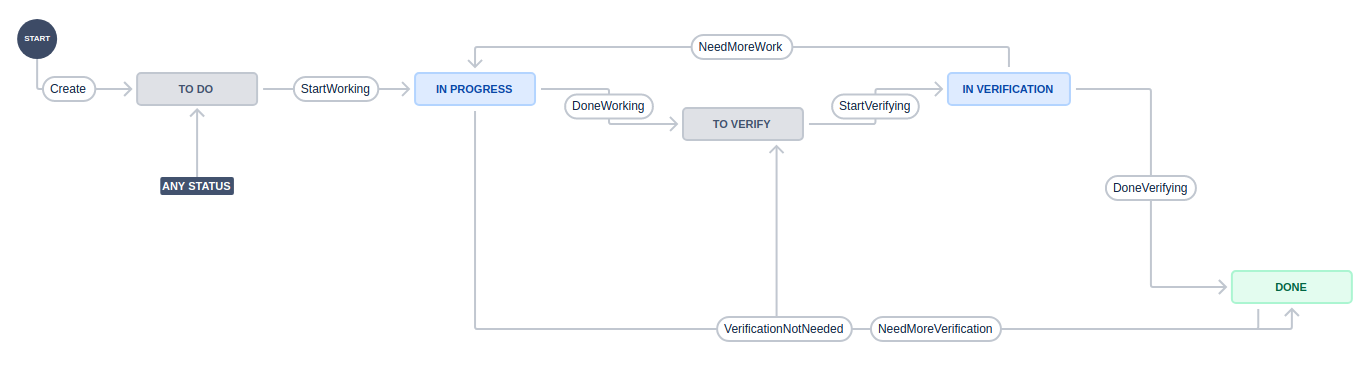
\includegraphics[scale=0.32]{res/images/jira_workflow.png}
            \caption{Diagramma degli stati e delle transizioni del workflow}
        \end{figure}
            Come si può vedere dall'immagine, il workflow di task\textsubscript{G} e sottotask è stato configurato di modo che ci siano delle precise transizioni da uno stato all'altro e che solo quelle siano permesse. I nomi delle transizioni sulle frecce corrispondono ai comandi da usare nella sintassi degli smart commit\textsubscript{G}. Maggiori dettagli si trovano nella wiki\textsubscript{G} \textsc{Git, Github \& Jira}.
        \pparagraph{Google Sheet}
        Si fa uso del foglio elettronico di Google Sheet per tenere traccia di tutte le informazioni relative alle metriche usate nel \textsc{Piano di Qualifica}. Contiene dati essenziali al controllo dello svolgimento del progetto, come il tempo per ogni lavoro individuale svolto dal singolo soggetto o il tempo effettivo e preventivato di una specifica riunione. Parte di questo foglio è stato bloccato in maniera tale da favorire l'inserimento dei soli dati da parte dei componenti del gruppo.
        
        \pparagraph{Google Sites}
        Collegato direttamente con i grafici del cruscotto presente in Google Sheet, il sito interattivo creato tramite Google Sites permette di avere una rapida visualizzazione dell'avanzamento del progetto. Questo sito, diviso in periodi, propone delle "fotografie" ritraenti degli specifici grafici utili a verificare velocemente metriche essenziali del \textsc{Piano di Qualifica} e la loro variazione tra periodi diversi.
        
        \pparagraph{Google Drive}
        Viene utilizzato uno spazio Google Drive per contenere tutti i file utili al gruppo, come presentazioni, materiale utile alla comprensione delle tecnologie da utilizzare, un foglio elettronico contenente le varie metriche per \textsc{Piano di Qualifica} e diagrammi \href{https://drawio-app.com/}{Draw.io}
        
        \pparagraph{Workflow per l'inizio di una nuova task}
        \begin{enumerate}
        	\item Si prende il codice della task da Jira: PCS-\#\#\# e si va sull’Excel \textbf{Sincronizzazione Dati} nella riga corrispondente \textbf{TEMPO (minuti) PREVENTIVATO} → tempo durata preventivato (relativo al lavoro);
        	\item in \textbf{ATA \#StartWorking → \#DoneWorking: }
        	\begin{itemize}
        		\item Settare date: \textbf{AVVIO} e \textbf{SCADENZA PREFISSATA};
        		\item Ogni qualvolta si committa con 'git commit -m “PCS-\#\#\# \#comment <commento> \#time <tempo>” ' (quindi usando tracciamento temporale di Jira) e si incrementa sull’excel.
        	\end{itemize}
        	\item Al termine del lavoro della task si dovrà andare ad inserire la data di fine effettiva della colonna \textbf{DATA \#StartWorking → \#DoneWorking FINE EFFETTIVA};
        	\item Aggiungere il \textbf{TEMPO (minuti) EFFETTIVO} con relativo \textbf{Ruolo};
        	\item quando finito controllare \url{https://threewaymilkshake.atlassian.net/wiki/spaces/VER/pages/138412040/Sequenza+Stesura+e+Verifica+verbali} e assegnare la verifica a chi tocca, secondo l’ordine.
        \end{enumerate}
    	
    	\pparagraph{Workflow per la verifica di una task}
    	\begin{enumerate}
    		\item Si prende il codice della task da Jira: PCS-\#\#\# e si va sull’Excel \textbf{Sincronizzazione Dati} nella riga corrispondente \textbf{TEMPO (minuti) PREVENTIVATO} → tempo durata preventivato (relativo alla verifica);
    		\item settare \textbf{SCADENZA PREFISSATA} in \textbf{DATA \#StartVerifying → \#DoneVerifying};
    		\item Al termine della verifica si dovrà andare ad inserire la data di fine effettiva della colonna \textbf{DATA \#StartVerifying → \#DoneVerifying AVVIO (=EFFETTIVA FINE DI \#TOVERIFY) FINE EFFETTIVA}.
    	\end{enumerate}
    
    	\pparagraph{Workflow per le riunioni}
    	Chi dovrà redigere il verbale dovrà::
    	\begin{enumerate}
    		\item In \textbf{Durata Riunioni - Dati} inserire la \textbf{Data, Prevista ed Effettiva}  sotto \textbf{Durata riunioni interne / esterne};
    		\item Creare branch feature/VT-n con T → {I, E}, n → numero
    		\item Quando finito, oltre a settare tempi come per task normali, controllare file in \url{https://threewaymilkshake.atlassian.net/wiki/spaces/VER/pages/138412040/Sequenza+Stesura+e+Verifica+verb} e:
    		\begin{itemize}
    			\item Spuntare la propria box;
    			\item Una volta che la task è in toVerify con l’assignee cancellato (si cancella da solo tramite automazione) assegnare a chi tocca la verifica.
    		\end{itemize}
    		\item Spostare note su Confluence → Trascritti.
    	\end{enumerate}

\subsection{I ruoli di progetto}
    La suddivisione in ruoli è necessaria per favorire la parallelizzazione e distribuzione del lavoro e delle responsabilità.
    \subsubsection{Analista}
    Hai il compito specifico di comprendere il problema. Ha un ruolo attivo fin quando la comprensione non è adeguata. Adottando un modello incrementale\textsubscript{G}, rimane più a lungo ed evolve. E auspicabile che ci siano più analisti per portare punti di vista diversi e sommare le conoscenze. Redige \textsc{Studio di Fattibilità} ed \textsc{Analisi dei Requisiti}.
    \subsubsection{Progettista}
    Traduce il problema in una possibile soluzione, descritta come architettura, divisa in parti per agevolare lo sviluppo individuale di queste. Dati i vincoli ha il compito di trovare una buona soluzione. Redige le specifiche tecniche e le definizioni del prodotto.
    \subsubsection{Verificatore}
    Agisce su ogni attività\textsubscript{G} ed attua una verifica oggettiva, segnalando eventuali problemi secondo il \hyperref[label]{text}{processo rispettivo}.
    \subsubsection{Programmatore}
    Implementa in codice ciò che i progettisti hanno definito come design. Un'adeguata divisione dei compiti tra diversi programmatori consente un alto parallelismo, ideale per avanzare rapidamente. Deve svolgere compiti piccoli, che siano facilmente verificabili.
    \subsubsection{Responsabile}
    Gestisce il controllo sul progetto\textsubscript{G} e tramite un cruscotto\textsubscript{G} di controllo aggiorna, revisiona ed adatta lo svolgimento dei lavori. Elabora piani e scadenze, assegna compiti, approva documenti, gestisce i problemi, redige l'\textsc{Organigramma} ed il \textsc{Piano di Progetto} ed approva l'offerta prima di sottoporla al committente.
    \subsubsection{Amministratore}
    Ha in carico la definizione, modifica ed agevolazione del way of working. È un percorso in logica JiT\textsubscript{A} procede per incrementi. È responsabile dell'efficacia e dell'efficienza nell'ambiente di lavoro, gestisce la documentazione, organizza il glossario, collabora alla redazione del \textsc{Piano di Progetto} e redige le \textsc{Norme di Progetto}.

\subsection{Gestione delle comunicazioni}
    Di seguito si definiscono le procedure e gli strumenti adottati per standardizzare ed organizzare le comunicazioni all'interno ed all'esterno del gruppo.
    \subsubsection{Comunicazioni interne}
        Riguardano i soli componenti del gruppo \group e in base allo scopo si articolano tramite strumenti diversi.
        \pparagraph{Google meet}
            Piattaforma di videoconferenze\footnote{\url{https://meet.google.com/}} di Google che permette la condivisione di più schermi e non richiede l'installazione di programmi aggiuntivi in quanto fruibile da browser. Integrata con Google Calendar permette la creazione di meeting collegati ad eventi direttamente da quest'ultimo strumento, semplificando così il processo di creazione ed organizzazione di eventi comuni.
            Viene utilizzata per le riunioni, le quali devono essere effettuate con una frequenza non inferiore a quella settimanale. Per ogni riunione il gruppo segue l'ordine del giorno che si sarà venuto a formare nel documento Confluence dedicato allo specifico incontro, al quale tutti possono collaborare. Le discussioni e le decisioni verranno raccolte dal segretario, che cambierà ad ogni riunione, per distribuire equamente questo compito a rotazione, nello stesso documento dal quale poi produrrà il verbale seguendo le regole definite in \ref{verbali}.
        \pparagraph{Slack}
            Strumento di messaggistica fortemente orientato alla collaborazione in gruppi di lavoro \footnote{\url{https://slack.com/intl/en-it/about}}. Il gruppo \group ha un workspace dedicato nel quale sono presenti diversi canali, per suddividere ed organizzare le comunicazioni. Durante lo svolgimento del progetto\textsubscript{G} si possono creare tanti canali quanti se ne rendono necessari, il responsabile provvederà alla gestione di questi. Oltre ai canali dedicati alle attività\textsubscript{G} appena citati ci sono i seguenti:
            \begin{itemize}
                \item \textbf{generale: }per le comunicazioni che non ricadono in nessun canale specifico già esistente e per le quali non si rende ncecessaria la creazione di un nuovo canale;
                \item \textbf{capitolato-c5-portacs: }all'interno del quale l'amministratore configura le integrazioni automatizzate utili a notificare i componenti del gruppo:
                \begin{itemize}
                    \item jira, invierà una notifica ogni qualvolta che si intraprenderà un'azione, manuale o automatica (\textit{smart commits}) sul cruscotto\textsubscript{G} di progetto\textsubscript{G};
                    \item github, notificherà ogni azione intrapresa sui branch \textit{master} e \textit{develop};
                    \item google calendar, che provvederà a notificare la programmazione di eventi e ricorderà quelli imminenti allegando codice Google meet per accedere direttamente alla riunione.
                \end{itemize}
            \end{itemize}
        \pparagraph{Telegram}
            Software di messaggistica \footnote{\url{https://telegram.org/}} nel quale il gruppo \group ha un gruppo dedicato utilizzato solamente per le comunicazioni informali e non strettamente legate al progetto\textsubscript{G} di lavoro.
    \subsubsection{Comunicazioni esterne}
        Possono avvenire tra il gruppo \group ed il proponente e/o con il committente. Il gruppo si adatterà allo strumento preferito da questi in ogni momento nel quale si renda necessario il contatto. Per le comunicazioni rapide e dirette che non richiedono un incontro sincrono fra le parti, fornitore e proponente si sono accordati per l'utilizzo di uno spazio Google Chat\footnote{\url{https://workspace.google.com/products/chat/}}.

\subsection{Gestione dei Rischi}
    \subsubsection{Descrizione}
        I rischi previsti o identificati devono essere prontamente documentati nel \textsc{Piano di Progetto}. Ogni rischio dovrà essere così descritto:
        \begin{itemize}
            \item nome;
            \item \textbf{codice}: secondo la classificazione in \ref{classifrischi};
            \item \textbf{occorrenza e pericolosità: }possono assumere i valori bassa, media alta;
            \item descrizione;
            \item metodologie di rilevamento;
            \item piano di contingenza.
        \end{itemize}
    \subsubsection{Classificazione dei Rischi}
    \label{classifrischi}
        Per facilitare raccolta e riferimenti successivi, il codice identificativo di ogni rischio deve seguire la seguente convenzione:
        $$ \text{RIS\_[tipo]-[num]} $$
        dove tipo può essere:
        \begin{itemize}
            \item \textbf{T} $\rightarrow$ tecnologico;
            \item \textbf{O} $\rightarrow$ organizzativo;
            \item \textbf{I} $\rightarrow$ interpersonale;
        \end{itemize}
    mentre num è un numero progressivo che parte da 1 per ogni categoria, ed è univoco all'interno della stessa.
    \begin{figure}[H]
        \centering
        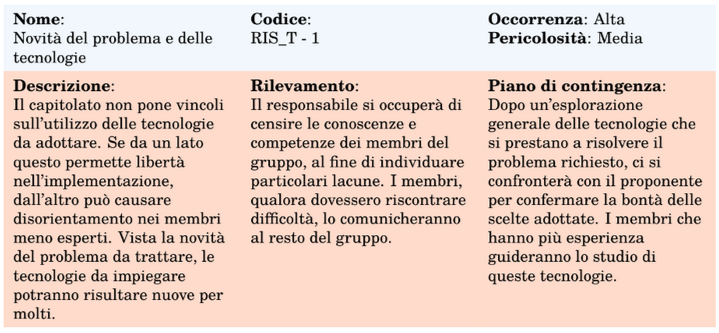
\includegraphics[scale=0.6]{res/images/esempio_rischio.png}
        \caption{Esempio corretto di raccolta rischio.}
    \end{figure}

\subsection{Formazione}
    I membri del gruppo \group sono tenuti a formarsi individualmente in quanto si ritiene che i tempi e le modalità di questo processo siano altamente individuali. Per quanto riguarda tecnologie e strumenti di interesse al gruppo, ogni membro è libero di creare una wiki\textsubscript{G} nello spazio dedicato di Confluence per raccogliere risorsa\textsubscript{G} e documentazioni utili, raccolte online o prodotte dallo stesso, così da condividere le proprie conoscenze apprese e velocizzarne l'assorbimento da parte degli altri componenti. \\
    Per i compiti attuali e per quanto discusso fino a questo momento con il proponente, si rimandano i membri del gruppo alle seguenti fonti ufficiali:
    \begin{itemize}
        \item \textbf{\LaTeX: }
            \subitem -- \url{https://www.latex-project.org/};
            \subitem -- \url{https://www.overleaf.com/learn};
        \item \textbf{Github: }\url{https://docs.github.com/en};
        \item \textbf{Confluence: }\url{https://confluence.atlassian.com/alldoc/};
        \item \textbf{Java: }\url{https://docs.oracle.com/en/java/};
        \item \textbf{Nodejs: }\url{https://nodejs.org/en/docs/}.
    \end{itemize}